51. $\cfrac{x^2-(\sqrt{3}+\sqrt{7})x+\sqrt{21}}{\sqrt{5-x}}\cdot\cfrac{x^2-4x+4}{6x-x^2-9}\leqslant 0\Leftrightarrow
\cfrac{(x-\sqrt{3})(x-\sqrt{7})(x-2)^2}{\sqrt{5-x}(x-3)^2}\geqslant 0.$ Применив метод интервалов, найдём ответ:
\begin{figure}[ht!]
\center{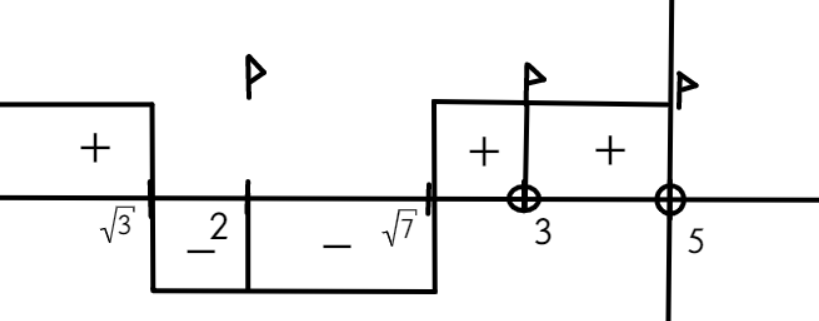
\includegraphics[scale=0.35]{int51.png}}
\end{figure}
$x\in(-\infty;\sqrt{3}]\cup\{2\}\cup[\sqrt{7};3)\cup(3;5).$\\
